\chapter{Cella solare}

\renewcommand\thesection{\Roman{section}}

\section{Rendimento di una cella solare}

\textbf{Obiettivo:} misurare l'efficienza di conversione fra l'energia elettrica prodotta da una cella solare e l'energia luminosa incidente.

\paragraph{Strumentazione:} 
\begin{enumerate}
    \item una cella solare;
    \item un banco ottico;
    \item un amperometro e un voltmetro. 
\end{enumerate}

\paragraph{Procedura:}
\begin{enumerate}
    \item disporre la cella sul banco ottico, il più possibile vicino alla lampadina, misurare la distanza pannello–filamento ed il diametro del pannello.
    \item costruire i circuiti: quello di sinistra è composto da un alimentatore di tensione continua in grado di fornire la potenza necessaria per alimentare la lampadina alogena;
    \begin{figure}[h]
        \centering
        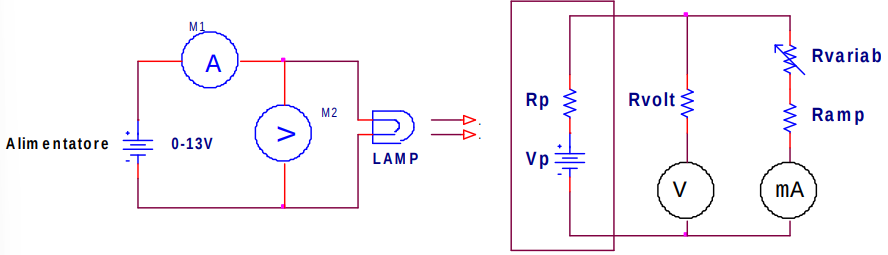
\includegraphics[width=0.9\linewidth]{Immagini/EXP8 - cella solare.png}
        \caption{circuiti per la lampadina alogena e la cella solare.}
        \label{fig: EXP8 - cella solare}
    \end{figure}
    \item alimentare la lampadina a $V_{gen}=\SI{12}{\V}$, leggere sul generatore di tensione in continua (o sul trasformatore) la corrente $I_{gen}$ che assorbe e la tensione e calcolare la potenza.
    \item effettuare le misure in avvicinamento;
    \item leggere la corrente $I$ indicata dal milliamperometro e la tensione $V$ sul voltmetro. Il rapporto fra tensione e corrente fornisce il valore della resistenza interna del milliamperometro, che non cambia, a meno di non cambiare scala allo strumento; in questo caso è necessario ripetere la misura;
    \item scollegare l'amperometro e leggere la tensione indicata: essa rappresenta la tensione $V_p$;
    \item osservare che la resistenza interna del pannello è di ordini di grandezza più piccola della resistenza del voltmetro;
    \item calcolare la resistenza $R_p$ della cella con i dati misurati di $V_p$, $I$ e $R_{amp}$;
    \item ricavare la corrente di cortocircuito della cella con $I_{cc}=V_p/R_p$;
    \item ricavare la potenza elettrica prodotta dalla cella con $P_{pannello}=I_{cc}V_p$;
    \item oscurare la luce che prodotta dalla lampada alogena incide direttamente sul pannello e misurare la potenza prodotta dalla luce di fondo $P_{fondo}$, ripetendo le misure da 4. a 8., la potenza generata dalla luce incidente sarà $P_{diretta}=P_{pannello}-P_{fondo}$;
    \item ripetere le misure da 4. a 9. per circo 10-15 distanze a intervalli di circa $\SI{5}{cm}$ l'una dall'altra e trovare la relazione tra l'efficienza e la distanza lampadina-pannello;
    \item graficare la corrente $I_{cc}$ e la tensione $V_p$ in funzione della distanza. Proporre un modello per interpretare i dati.
\end{enumerate}

\section{Caratteristica I-V di una cella solare}

\textbf{Obiettivo:} verificare il teorema del massimo trasferimento di potenza tramite l'aggiunta di un reostato e determinare la caratteristica I-V della cella.

\paragraph{Strumentazione:}
\begin{enumerate}
    \item un reostato;
    \item gli elementi della parte precedente.
\end{enumerate}

\paragraph{Procedura:}
\begin{enumerate}
    \item disporre la cella a una certa distanza dalla lampadina, non troppo vicina per evitare effetti termici (noi avevamo scelto il più lontano possibile);
    \item ATTENZIONE! Prima di procedere calcolare $R_{amp}$ e $R_{p}$ e assicurarsi che $R_p>R_{amp}$;
    \item determinare il range della resistenza di carico $R_{var}$;
    \item ripetere le misure da 4. a 8. (della parte I) facendo variare $R_{var}$;
    \item non è necessario fare le misure in oscuramento e si può fare un'unica misura di $V_p$ (step 5. della parte I);
    \item graficare la caratteristica $I(V)$ della cella;
    \item graficare la potenza fornita al carico (composto dalla $R_{var}$ e dalla resistenza $R_{amp}$). Se il modello proposto è corretto dovrà risultare un massimo della potenza trasferita per $R_p=R_{var}+R_{amp}$.
\end{enumerate}

\setcounter{section}{0}
\renewcommand\thesection{\Alph{section}}

\section{Considerazioni geometriche}
Per calcolare l'efficienza di conversione della cella elementare è necessario calcolare il rapporto fra la potenza incidente sulla cella e la potenza elettrica prodotta dal pannello. La potenza incidente sul pannello è ricavabile dall'angolo solido $\Omega$ sotteso dal pannello solare. Dato che
\begin{equation}
    \Omega=\int_{0}^{2\pi}d\phi=\int_{0}^{\theta}\sin{(\alpha)}\,d\alpha=2\pi(1-\cos{\theta}),
\end{equation}
e che la lampadina emette su tutto l'angolo solido di $4\pi$, la potenza che arriva sul pannello è la frazione $\Omega/4\pi$, quindi
\begin{equation}
    P_{incidente}=\frac{1-\cos{\theta}}{2}P_{lampadina},\quad P_{lampadina}=I_{gen}V_{gen}.
\end{equation}
Indicando con $r$ il raggio del pannello si può scrivere
\begin{equation}
    \cos{\theta}=\frac{d}{\sqrt{r^2+d^2}}.
\end{equation}
L'efficienza del pannello, in funzione della distanza $d$, è
\begin{equation}
    \eta=\frac{P_{diretta}}{P_{incidente}}.
\end{equation}
Nel caso in cui la sorgente luminosa è molto
distante dai pannelli, è possibile semplificare le relazioni tra potenza incidente e potenza prodotta approssimando la superficie del pannello ad una calotta sferica. In questo caso se $r\ll d$ si può approssimare
\begin{equation}
    \cos{\theta}=\frac{d}{\sqrt{r^2+d^2}}\approx 1-\frac{1}{2}\frac{r^2}{d^2}.
\end{equation}